本次完整运行的主结果为600张图全部匹配正确，ACC=100\%、ARI=1、NMI=1，六个预测簇各有100张。数据核查确认全部图像可读取，600个文件哈希互异，未发现像素完全相同的重复图片。

\begin{center}\small
\begin{tabularx}{\linewidth}{Xrrrr}\toprule
方案 & 运行数 & ACC（\%） & ARI & NMI\\\midrule
颜色纹理＋K-means & 5 & $100\pm0$ & $1\pm0$ & $1\pm0$\\
ResNet18＋K-means & 5 & $100\pm0$ & $1\pm0$ & $1\pm0$\\
ResNet18＋PCA64＋K-means & 5 & $100\pm0$ & $1\pm0$ & $1\pm0$\\
ResNet18＋Ward & 1 & 100 & 1 & 1\\\bottomrule
\end{tabularx}\end{center}

前三行是五个预定种子的均值和样本标准差，最后一行是确定性算法的单次结果。三个K-means方案各自的十对种子间ARI均为1，说明这些运行得到相同的样本分组，仅簇编号可能不同。

\textbf{最重要的结论是简单基线已经足够。}这批图片的类别差异在传统颜色和纹理表示中已经可以分离。实验没有提供深度特征优于传统特征的外部指标证据，也没有显示PCA或Ward进一步提高正确率。主方法保持预先声明的深度特征方案，并不在看过标签后重新选择“最漂亮”的模型。若以完成当前分组为唯一目标，传统方案也能满足要求；更复杂表示的优势需要另一个更有挑战、预先定义的数据条件来检验。

PCA64保留归一化深度特征约97.34\%的方差，维度由512降到64，外部指标不变。手工、深度、PCA空间中的轮廓系数分别为0.8374、0.6783、0.7203；由于空间不同，不能据此直接排列语义性能。深度K-means与Ward使用相同空间且得到相同分组，因此两者轮廓系数同为0.6783。

全部图像的读取、校验和两类特征提取合计约54.59秒，运行于CPU四线程环境。该计时包含两类表示，不是单独ResNet的速度测试。机器、库版本、线程数和缓存都会影响时间。记录中保留了实际环境和权重哈希。

12项评价单元测试已通过；独立核验进一步检查全部16组指标、15组K-means最近中心分配、PCA重建以及保存文件一致性。外部指标全部达到上限，仍然不意味着对新背景、新拍摄条件、未见产品或有缺陷图像也能完美分组。原图背景和纹理与类别相关，这可能使当前任务较易，但本实验没有通过专门干预证明这种因果解释。

\IfFileExists{../course-report/figures/method-overview.pdf}{%
\begin{figure}[H]\centering
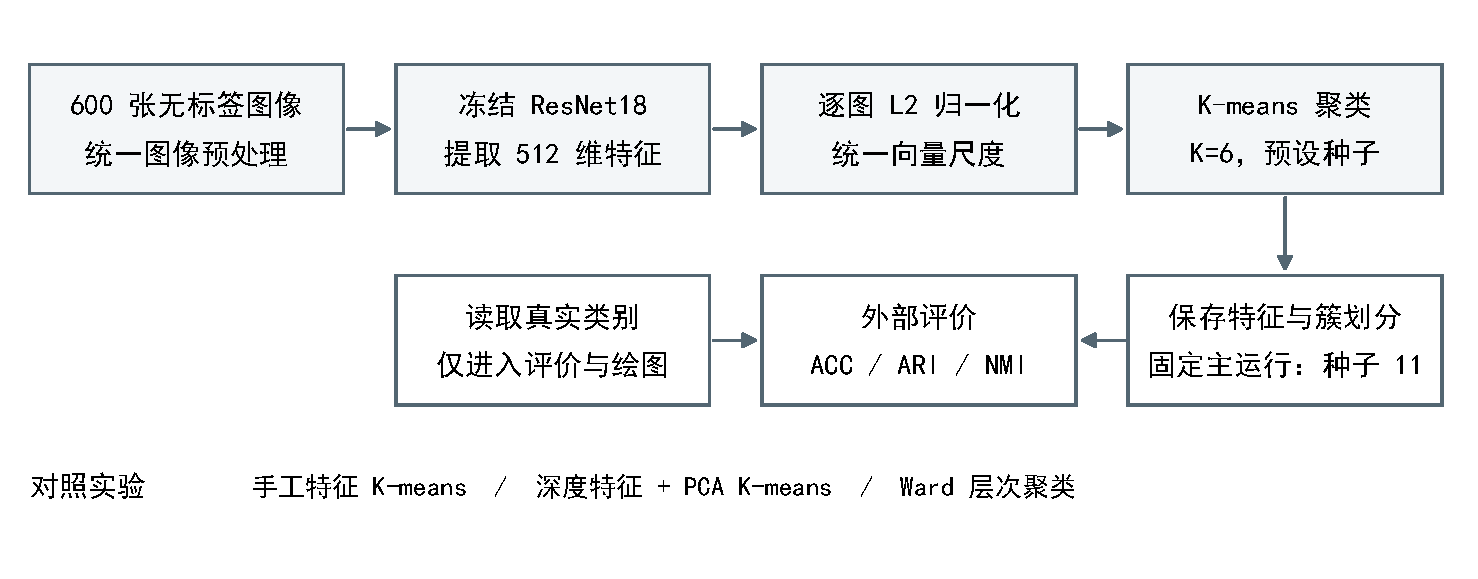
\includegraphics[width=\linewidth]{../course-report/figures/method-overview.pdf}
\caption{第一题主方法与评价边界。真实类别不进入特征提取和聚类。}
\end{figure}}{}
